\documentclass[../../../../projectPlan.tex]{subfiles}

\begin{document}

	\section{Project Effort and Cost}

		To make an Effort estimation we have to compute this formula:

		\[effort = 2.94 * EAF * (SLOC/1000)^E\]

		Where:
		\begin{itemize}
			\item \(effort\) is the value to estimate.
			\item \(2.94\) is a constant defined by COCOMO II 2000.0.
			\item \(EAF\) is the "Effort Adjustement Factor" calculated in the following sections.
			\item \(SLOC/1000\) that is the KSLOC (Kilo SLOC) number.
			\item \(E\) that is an exponent calculated in the following sections.
		\end{itemize}

		\subsection{Computation of \(E\) parameter}
			The parameter \(E\) is calculated as:
			\[E = B + 0.01 * SFs\]
			Where:
			\begin{itemize}
				\item \(B\) is a constant given by the COCOMO II and his value is 0.91.
				\item \(SFs\) is an aggregation of five Scale Factors described in the document at \url{http://csse.usc.edu/csse/research/COCOMOII/cocomo2000.0/CII_modelman2000.0.pdf}
			\end{itemize}
			

			The following table contains the variuos values for these Scale Factors (table taken from the previous URL).

			\begin{figure}[H]
				\centering
				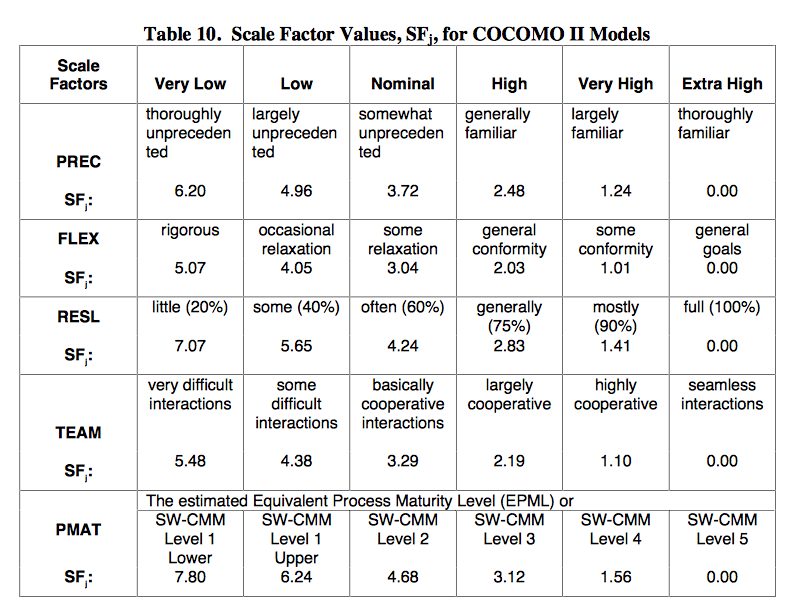
\includegraphics[width=\textwidth, scale=0.5]{../images/ftable.png}
			\end{figure}

			\begin{itemize}
				\item \textbf{PREC} (Previous experience of the organization with these type of projects): LOW (4.96).
				\item \textbf{FLEX} (Degree of flexibility in development process): HIGH (2.03).
				\item \textbf{RESL} (Risk Analysis): HIGH (2.83).
				\item \textbf{TEAM} (How well the development team knows each other): EXTRA HIGH (0.00).
				\item \textbf{PMAT} (Maturity of the Organization): NOMINAL (4.68).
			\end{itemize}

			The result is the sum of these factors:
			\[SFs = \sum_{j=1}^{5} SF_j = 14.67 \]

			So we can now compute the \(E\) parameter:
			\[E = B + 0.01 * SFs \\
			    = 0.91 + 0.01 * 14.67
			    = 1.558\]

		\subsection{Computation of \(EAF\) parameter}
			All the parameters discussed in this paragraph are described in section 3.2 of the document at this URL: \url{http://csse.usc.edu/csse/research/COCOMOII/cocomo2000.0/CII_modelman2000.0.pdf}

			\begin{itemize}
				\item \textbf{Required Software Reliability (RELY)}
				      The results of a failure in our system is easily recoverable (e.g. loss of priority in the zone queues) so the RELY factor is LOW (count as 0.92).

				\item \textbf{Data Base Size (DATA)}
				      The effort needed to assemble and maintain the data required to complete test of the program is such that the DATA factor is NOMINAL (count as 1.00).

				\item \textbf{Product Complexity (CPLX)}
				      The area of our project is "Data Management" and the complexity is HIGH because we have simple triggers activated by data stream contents and complex data restructuring (e.g. maintain the zone queues updated) (count as 1.17).
				
				\item \textbf{Developed for Reusability (RUSE)}
				      This factor accounts for the additional effort needed to construct components intended for reuse on current or future projects. We think that we only have to design modules for the internal reuse in the myTaxiService system, so the descriptor is: NOMINAL (count as 1.00).
				
				\item \textbf{Documentation Match to Life-Cycle Needs (DOCU)}
				      We think that the documentation we have to produce is necessary in function of the lifecycle of the system, so we assign to DOCU the NOMINAL level (count as 1.00).
				
				\item \textbf{Execution Time Constraint (TIME)}
				      Our system is supposed to be fast because it's a Taxi reservation system, so the system is supposed to occupy less than 50 percent of the available execution time.
				      The label for TIME is NOMINAL (count as 1.00).
				
				\item \textbf{Main Storage Constraint (STOR)}
				      Due to the fact that the web application does not occupy the user's memory and that the mobile application is relatively simple, we only have to consider the memory occupation on the server side. This memory occupation change in function of the number of the users and increments if the usage of the system is high. We have to consider many things like Server Software, External API implementation, Database Space, so the label for TIME is HIGH (count as 1.05).
				
				\item \textbf{Platform Volatility (PVOL)}
				      Due to the fact that we have to implement a Mobile Application and a Web application, and the technologies we have to use (Android, iOS, Windows Phone programming languages, JS Frameworks for the website) receives continuous updates, we have to consider the PVOL facor at least NOMINAL (count as 1.00).
				
				\item \textbf{Analyst Capability (ACAP)}
				
				\item \textbf{Programmer Capability (PCAP)}
				
				\item \textbf{Personnel Continuity (PCON)}
				
				\item \textbf{Applications Experience (APEX)}
				
				\item \textbf{Platform Experience (PLEX)}
				
				\item \textbf{Language and Tool Experience (LTEX)}
				
				\item \textbf{Use of Software Tools (TOOL)}
				
				\item \textbf{Multisite Development (SITE)}
				
				\item \textbf{Required Development Schedule (SCED)}

			\end{itemize}

\end{document}